\chapter{Survey layout and Questions}


These were the questions and answer options as used in Nettskjema survey. This was accessed via a specially created website, which had full details about the research and the ability to contact the researcher. 
https://aamccormack12.wixsite.com/sealevelextremes 

The survey was designed for access via smartphones, computers and tablets. The UI was checked on each of these machines and the first targeted recipients course mates and then test engineers, so that any issues could quickly be discovered and fixed. 

\section{Example Survey - Grillstad English}

Do you consent to these answers being used for an MSc research project?
\begin{itemize}
	\item Yes
    \item No
\end{itemize}

\paragraph{}
How long have you known this area?
\begin{itemize}
	\item > 30 years.
    \item > 20 years
    \item > 10 years
    \item > 5 years
    \item > 1 year
    \item < 1 year
\end{itemize}

\paragraph{}
What communities in this area are you part of?
\begin{itemize}
    \item marine worker
    \item non-marine worker
    \item resident
    \item student
    \item leisure user - land
    \item leisure user - water
    \item commuter
    \item other 
\end{itemize}
Other (Write in here)
\paragraph{}

This research investigates knowledge about extreme sea levels in Trondheim, focusing on storm surges. A storm surge occurs when the weather temporarily causes water to be forced up and onto the coast.

A 20-year storm surge refers to the probability of an event, meaning there is a 1 in 20 chance (5%) of this level of event every year. This expectation changes over time, for example due to climate change.

What is your level of interest in sea level extremes?
\begin{itemize}
    \item professional interest
    \item high
    \item medium
    \item low
    \item low
    \item not interested
\end{itemize}
\paragraph{}

The following questions display simulated water levels extremes in Trondheim. The numbers in these images refer to the height above NN2000 which can be considered an approximation of mean sea level.
\paragraph{}
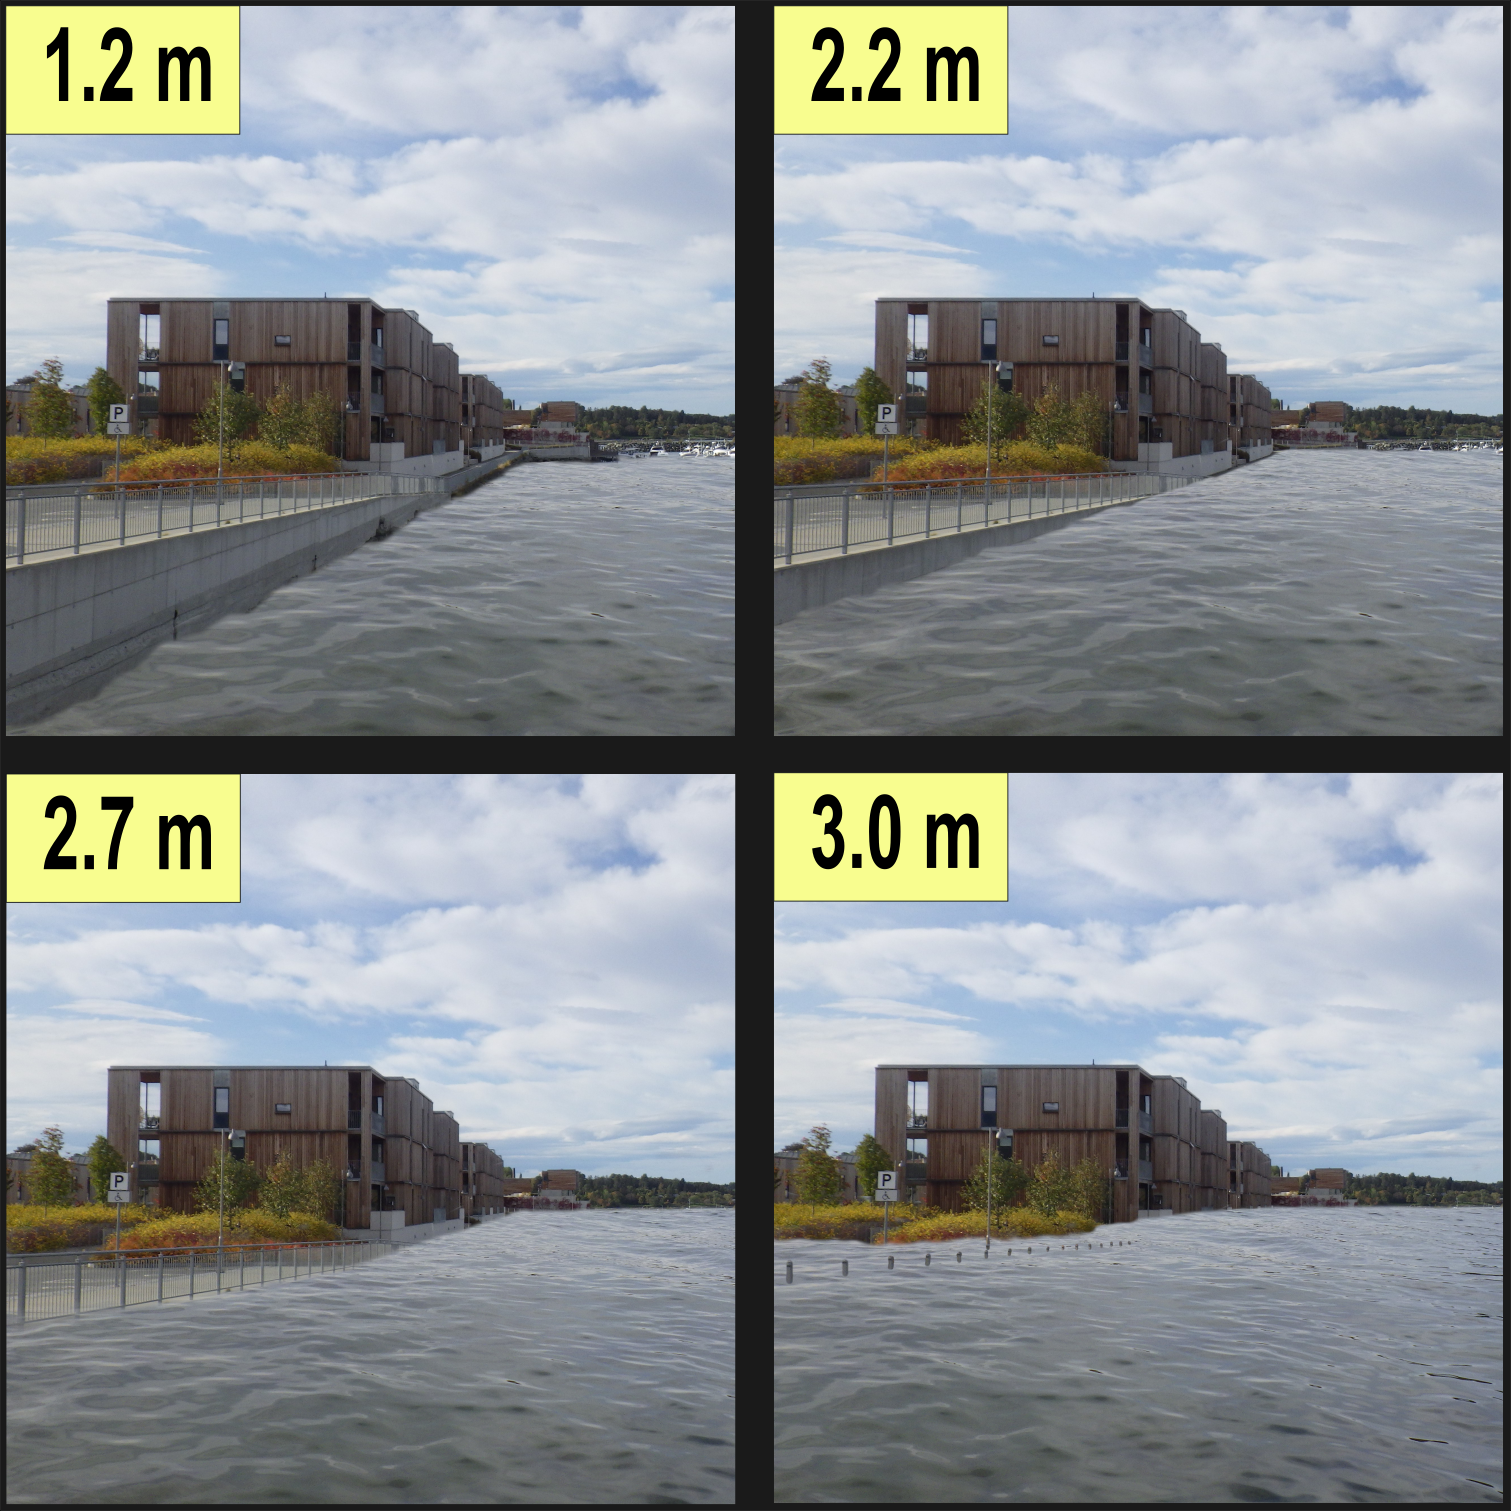
\includegraphics[width=1\textwidth]{fig_appendix/grillstad 2090 q.png}

Which image shows the current 20-year storm surge?
\begin{itemize}
    \item 1.2 m
    \item 2.2 m
    \item 2.7 m
    \item 3.0 m
\end{itemize}
\paragraph{}

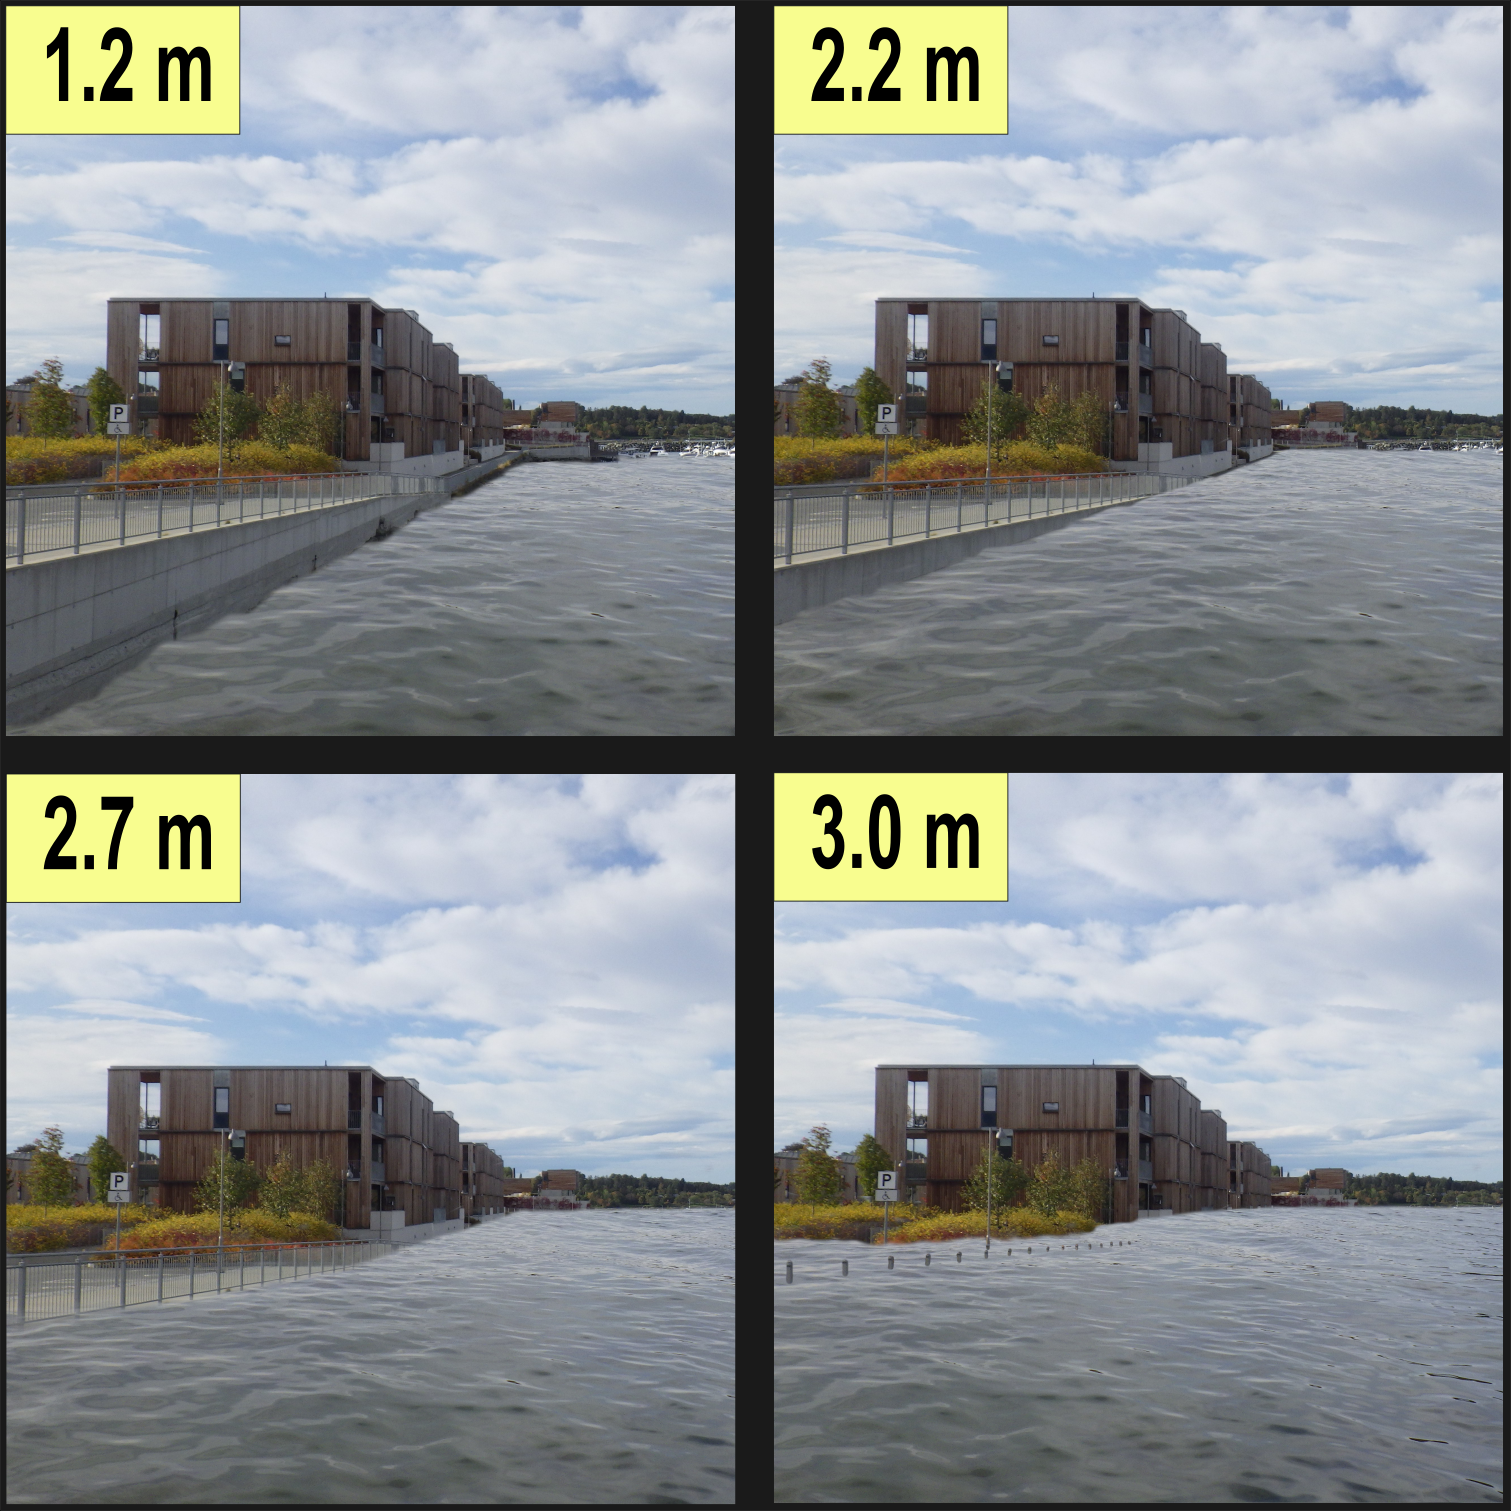
\includegraphics[width=1\textwidth]{fig_appendix/grillstad 2090 q.png}
Which image shows the 20-year storm surge projected for 2090?
\begin{itemize}
    \item 1.2 m
    \item 2.2 m
    \item 2.7 m
    \item 3.0 m
\end{itemize}
\paragraph{}

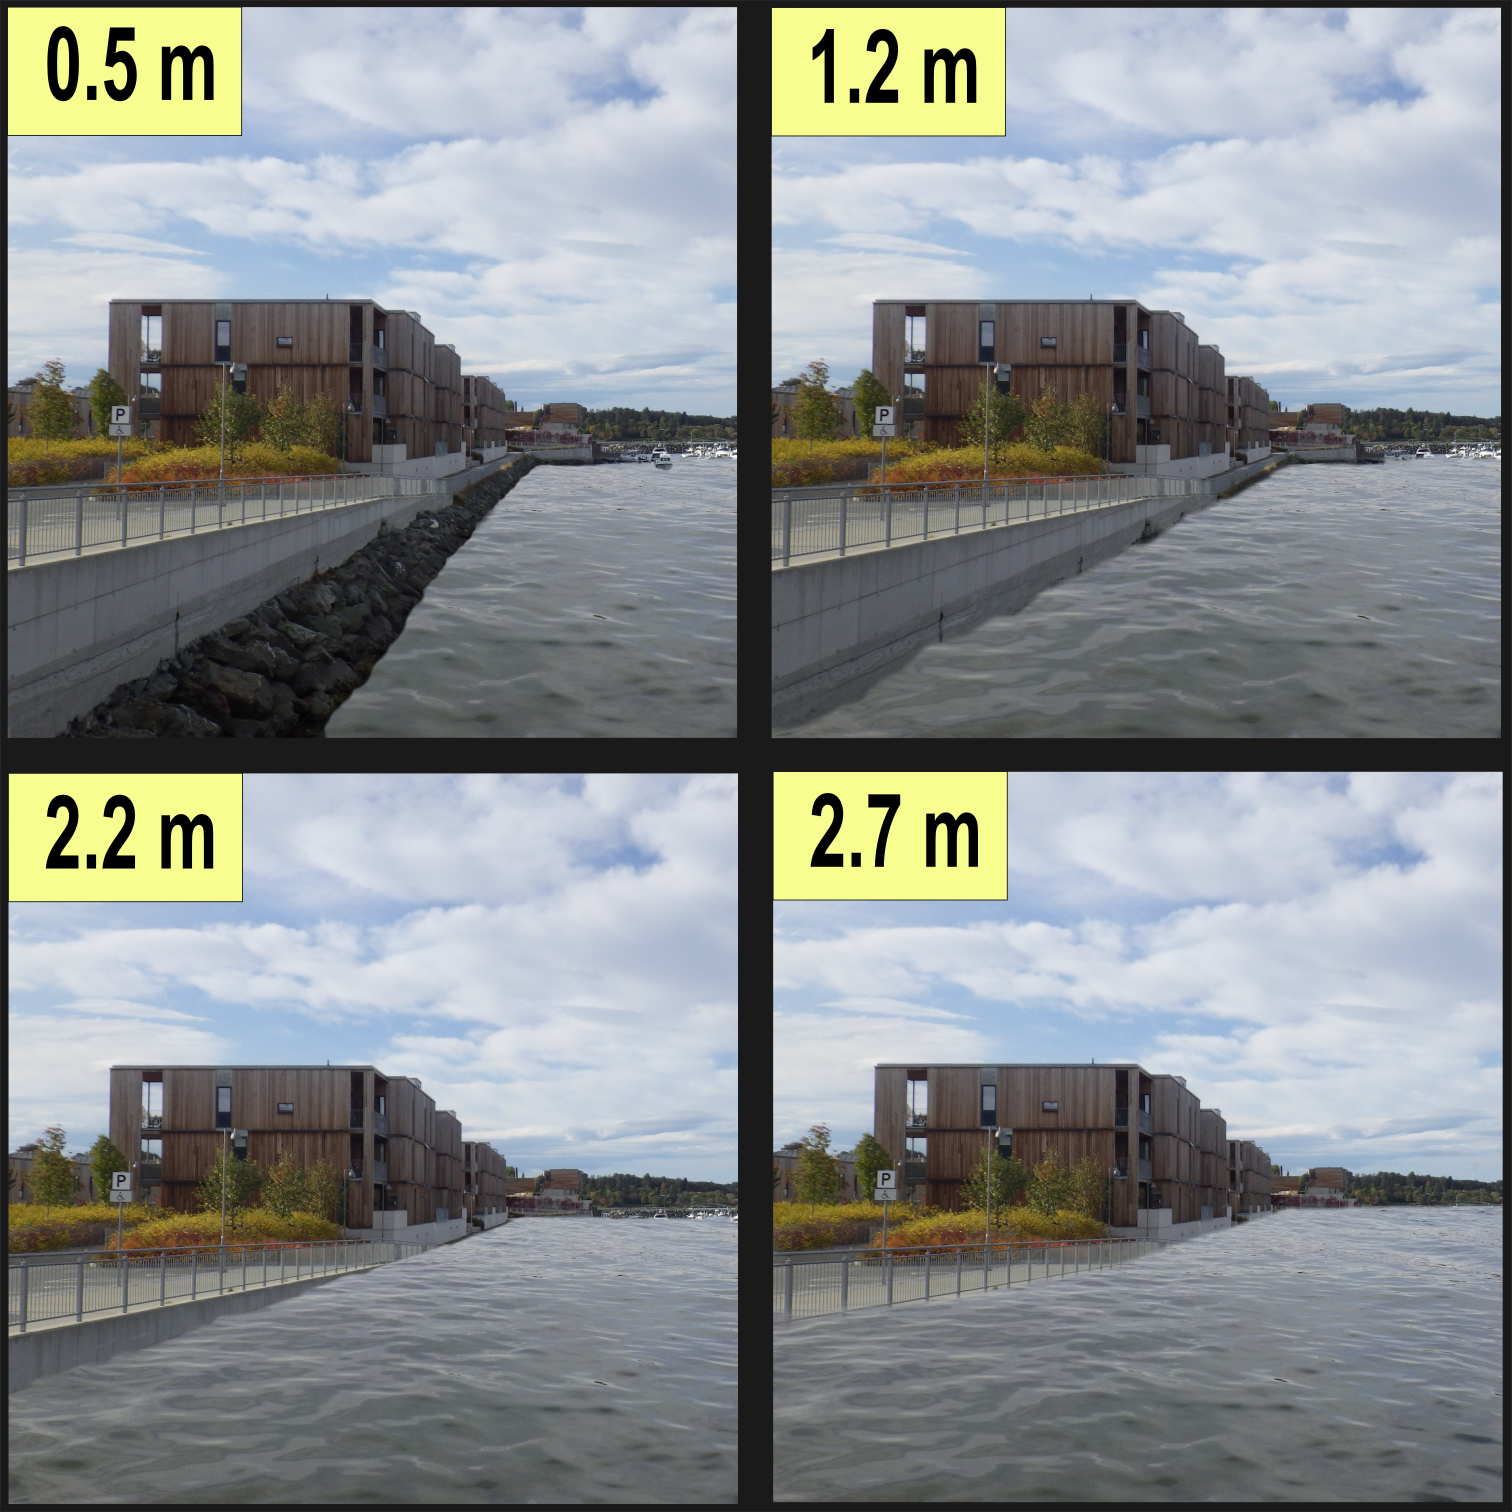
\includegraphics[width=1\textwidth]{fig_appendix/grillstad 2022 q.png}
Which image displays the current high tide?
\begin{itemize}
    \item 0.5 m
    \item 1.2 m
    \item 2.2 m
    \item 2.7 m
   \end{itemize}
\paragraph{}

Where do you get information about changes to this place?
e.g. subsidence, incidents, roadworks
\begin{itemize}
    \item personal observation
    \item family
    \item friends
    \item newspapers
    \item tv
    \item social media
    \item organisation membership
    \item municipality
\end{itemize}
\paragraph{}

Where do you get information about climate change?
\begin{itemize}
    \item personal observation
    \item family
    \item friends
    \item newspapers
    \item tv
    \item social media
    \item organisation membership
    \item peer-reviewed articles
    \item formal education
\end{itemize}

\paragraph{}
Are you concerned about climate change?
1 - not at all, 5 - very concerned
Rating Scale

\paragraph{}
How would flooding associated with sea level extremes in this area affect you?
\begin{itemize}
    \item no impact
    \item mild impact
    \item medium impact
    \item significant impact
\end{itemize}
If you would like to give more details on this, please write below.
\paragraph{}

How much do you think the sea level has changed here in the past 30 years?
\begin{itemize}
    \item + 50 cm
    \item + 20 cm
    \item + 10 cm
    \item no change
    \item - 10 cm
    \item - 20 cm 
    \item - 50 cm 
\end{itemize}
\paragraph{}

How much do you think the sea level will change in the next 30 years?
\begin{itemize}
    \item + 50 cm
    \item + 20 cm
    \item + 10 cm
    \item no change
    \item - 10 cm
    \item - 20 cm 
    \item - 50 cm 
\end{itemize}
\paragraph{}

Please tick if you remember any of these dates when coastal sea levels in Trondheim were over 2m.
\begin{itemize}
    \item 2020 February
    \item 2011 November
    \item 1999 November
    \item 1998 February
    \item 1997 February
    \item 1993 January
    \item 1990 February
    \item 1971 November
    \item I do not remember any of these events
\end{itemize}
\paragraph{}

From the following what are the major risks to people in this area?
\begin{itemize}
    \item shoreline instability
    \item storm surges
    \item waves
    \item strong winds
    \item strong tides
    \item drowning
    \item cold water shock
    \item I don't know
    \item I perceive no major risks
    \item human error
\end{itemize}
\paragraph{}

From the following what are the major risks to infrastructure in this area?
\begin{itemize}
    \item shoreline instability
    \item storm surges
    \item waves
    \item strong winds
    \item strong tides
    \item I don't know
    \item I perceive no major risks
    \item weathering
    \item precipitation
    \item human error
\end{itemize}

\paragraph{}
If you would like to give other examples of risk in this area, please write here.
\paragraph{}

How did you access this survey?
\begin{itemize}
    \item poster
    \item email
    \item social media
    \item via organisation membership
    \item via place of employment
    \item personal connection to researcher
\end{itemize}
\paragraph{}

If you would like further information on this research, please provide your e-mail address.

%have so far just written out English survey - if totally stuck can also do the norwegian one

%%%%% example bullet point
\begin{itemize}
	\item This is a bullet point.
    \item This is another one.
\end{itemize}

Here is some stuff I really need enumerated:

\begin{enumerate}
	\item This is the 1st item.
    \item This is the second item.
\end{enumerate}

\section{Example Survey - Nidelva Norwegian }